\section{Method}\label{6_method}
\begin{comment}
-- briefing
-- methods
-- pre-/post measurement
-- execution
-- interview
\end{comment}
\subsection{Conditions of Slackline Training}
Each participant is provided with the same levels, exercises and its detailed description about the execution.
The difference in each conditions lies in the training method itself, how the information is provided to the participant, and how feedback about the execution is given.
In the following each condition is described as well as the apparatus.

\subsubsection{Interactive System Group}
The participant interacts on her own with the system, which teaches the user how to interact with it and guides her through predefined exercises.
It explains on its own how to execute the exercises with a detailed description and a looping video.
Furthermore, how many repetitions and in which time to accomplish each repetition.
It provides real-time feedback about the current execution performance with several indicators.
If the exercise is too difficult to accomplish or not recognised by the system, the participant has the possibility to skip it.
Since its a think-aloud study, the participant further tells on which actions she is troubling with and when there is any confusion or misunderstanding with the system implementation.
%The experiment leader had no influence about questions regarding the exercise execution to ensure the autonomy of the user with the system.

\subsubsection{Human Trainer Group}
The participant is instructed by a human trainer, which in this case is the director of the study.
At first the trainer provides an instruction about the ongoing level of exercises.
Then the specific exercise is instructed. How to execute the exercise, how many repetitions, and the minimum time the trainee should hold the pose.
After that the trainer demonstrates the execution of the exercise for the trainee.
The trainer himself has an exercise description sheet to provide the trainee with the same information as the ISG.
\begin{figure}[htb]
	\centering
	\begin{minipage}[t]{1\linewidth}
		\centering
		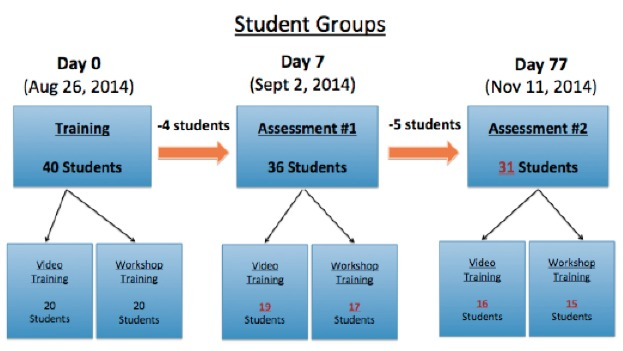
\includegraphics[width=0.8\linewidth]{Pictures/6_studyGroupsExample}
		\caption{Study groups example}
		\label{fig:6_studyGroups}
	\end{minipage}
\end{figure}

\subsubsection{Apparatus}
Figure \todo{[figure]} shows the setup of the study.
The Kinect was attached on a tripod with a height of \todo{90 cm}.
It is placed in front of a wall, which is used as projector screen.
The camera is faced in the direction of the slackline.
A projector is mounted on the ceiling of the room to project the systems interface on a wall.
The mobile slackline stands, like discussed in Section~\ref{5_1_hardwareComponents}, directly in front of the Kinect.
Marker attached on the slackline provide information for pre- and post-measurements as well as the starting point for the participant to get up the line.
The set up for the human trainer group was the same, but without the projector and the Kinect.
To record the execution a video camera was placed behind the participant to have her actions as well as the interface interaction recorded.
The set up was not changed during the study to have the same condition for every participant.

\todo{[Figure]}

\subsection{Design and independent \& dependent variables}\label{6_variables}
The experiment of the study is a 2 x 2 mixed factorial design.
Subjects were randomly assigned to a interactive system group (experimental) or a human trainer group (control).
Within subject a pre-measurement and post-measurement was conducted.
The measurements are divided into two parts.
First, measuring the time of a single leg stance with the left as well as the right foot on the slackline.
Second, measuring the steps and distance the participant can walk on the slackline with the left and right foot as starting point.
The distance and steps on the slackline were measured by dividing the mobile slackline into five areas, each with a distance of 60 cm.
Three attempts per side of the foot and method were executed and calculated to compare the results.

\textbf{Independent variables}
\begin{itemize}
\item Interactive Slackline Group
\item Human Trainer Group
\end{itemize}

\textbf{Dependent variables}
\begin{itemize}
\item Time stood on line with left, right, both feet
\item As many steps as possible on the line ( + distance with markers on the line) left, right feet
\item Accomplished exercises
\end{itemize}

\textbf{Confounding variable}
\begin{itemize}
\item Experience with general balance training
\item Experience with slacklining
\item General physical activity
\end{itemize}

%A measurement of the participants' current balance performance was conducted before and after the training to compare the training results and learning progress.  This involves the measurement of how long the participant can stand on the slackline in seconds with her left, right, and with both feet. Further, how many steps were she able to walk on the slackline with the left or right foot for getting up the line. Three attempts per side and method were executed and \todo{the best taken / the average calculated} to compare the results.

\begin{comment}
2 x 2 mixed factorial design
2 within subject --> test
pre-test
post-test

2 between subject --> training
Experiemental group --> ISG
Base line group --> HTG

ODER

3 dependent vs 2 independent variables
\end{comment}

\subsection{Procedure}
At first the participant was welcomed and then briefed about the idea as well as what she can expect from the study. Further an introduction about the training method in which she participates was given. After that she had to fill out a questionnaire for collecting demographic data and her prior experience with slacklining. The ISG had to answer one more question about the prior experience with interactive devices (e.g. Kinect, Wii, PlayStation Move, etc.).
%Therefore one can see if a person, which tends to have a better experience with the system during the study, relies on her prior experience with such devices. 
The physical activity level as well as the lateral preference was determined like stated above. Lastly she had to confirm a form consent.

\todo{pre-measurement eher allgemein halten und in 6.3.4 ausarbeiten oder testprozedere hier näher erläutern (attempts, wie lange maximal, marker an der slackline, etc.), oder reicht das?}

The general balance ability of the participant was obtained before training by how long she can stand on the ground and a towel.
Further, a pre-measurement of the slackline balance ability and the steps the participant is able to go on a slackline was conducted for comparison in a post-measurement.
%Here the participant had to balance a single leg stance on the slackline with the left as well as with the right foot.
%The time was counted if the balancing leg of the participants leaves the ground and stopped if she gets in contact with the ground with any foot.

After finishing the pre-measurements the participant was introduced about the ongoing training method.
She had to stay on a marked position on the ground and on the slackline, which gives the starting position for all exercises. 
She had to execute all exercises either provided by the system or the trainer.
These are divided into four levels with \todo{6, 4, 6, and 3 exercises}.
Between each exercises the participant could take a break if desired.

After the training the participant was asked to rank the difficulty of the exercise from a range of 1 (very easy) to 5 (very difficult).
Therefore the ranking of the participant can be compared with the logged performance data.
Hereby, it can be shown if the difficulty of the exercise set in each level is increasing and match the users' assumptions. %integrated exercise routine.

\todo{post-measurement eher allgemein halten und in 6.3.4 ausarbeiten oder testprozedere hier näher erläutern (attempts, wie lange maximal, marker an der slackline, etc.)?}

When finished with the training a post-measurement was conducted with the same procedure, like seen above in the pre-measurement.

Finally the participant had to answer questions a semi-structured interview to obtain her opinion on the general method and application scenarios for exactly this method with the slackline and other sport activities that could fit this method. The ISG were additionally interviewed about the user interface of the SLS and their experience with the interaction. The specific questions can be seen in \todo{Appendix}.
%for reviewing and validating performance parameters as well as to detect system failures.


